It looks like the way forward on the streaming channel project is that I
will need to recruit a board of control. Yeah, I cannot run the thing
solo. I am no
\href{https://en.wikipedia.org/wiki/Benevolent_dictator_for_life}{``Benevolent
Dictator For Life''}. Television, regardless of the transmission medium,
requires the work of many to make it work. It would be nice to offload
the administrative stuff and just focus on the tech, too.

Considering the bias locally against sole proprietors I would have to do
this anyhow. There is nice guidance from
\href{https://www.ohiosos.gov/businesses/information-on-starting-and-maintaining-a-business/starting-a-business/}{the
Ohio Secretary of State} as to bootstrapping a business. There is also a
guide on
\href{https://www.ohiosos.gov/globalassets/publications/busserv/llc.pdf}{how
to make an LLC in this state from the Secretary of State's office}.
There is a difference between impossibility and just being a pain in the
butt to organize. Hopefully I can recruit some initial board members who
agree with the vision of getting this started.

Properly launching efforts by Easter would be nice. Might it be
possible? We'll need \href{https://nextcloud.com/talk/}{Nextcloud Talk}
as well as \href{https://nextcloud.com/groupware/}{Nextcloud Office} as
well as
\href{https://www.collaboraoffice.com/collabora-online/}{Collabora
Online} for a small/medium business back-end bit of infrastructure.
Yeah, we would need \href{https://nextcloud.com/hub/}{Nextcloud Hub} and
\href{https://www.collaboraoffice.com/collabora-online/}{Collabora
Online} as well as plenty of storage space so that we could work around
the lack of an in-person workspace. At least one perpetual license for
\href{https://www.videostudiopro.com/en/licensing/business/}{Corel
VideoStudio Pro} would be beneficial as not everyone would be willing to
work with \href{https://kdenlive.org/en/}{kdenlive} or
\href{https://www.openshot.org/}{OpenShot}. We'd have to invest in a CDN
eventually which would likely mean getting set up with
\href{https://vimeo.com/ott/resources/}{Vimeo}. Various bits of gear
such as
\href{https://www.bhphotovideo.com/c/products/Pro-Camcorders-Cameras/ci/1881?sort=PRICE_LOW_TO_HIGH&filters=fct_a_features_2248\%3Alive-streaming-capability\%2Cfct_digital-interface_2247\%3Ahdmi\%7Cusb-c\%2Cfct_mic-input-hidden_6493\%3A3.5mm\%2Cfct_sensor-size_7003\%3A1-2.3in\%7C1-2in\%7C1-inch\%2Cfct_system-type_2110\%3Antsc}{cameras},
\href{https://www.bhphotovideo.com/c/search?q=camcorder\%20mic&sort=PRICE_LOW_TO_HIGH&filters=fct_a_power-source_1353\%3Abattery\%2Cfct_category\%3Ashotgun_8533\%2Cfct_connector-type_4116\%3A1-8in-mini\%2Cfct_integrated-mount_7062\%3Ayes\%2Cfct_stereo-mono_1411\%3Astereo}{microphones},
and lighting would need procuring too. Proper ``work'' computers would
be needed from either
\href{https://www.bhphotovideo.com/c/products/Windows-Computers/ci/16360/cp/28407\%2B50992\%2B16360?sort=PRICE_LOW_TO_HIGH&filters=fct_a_wireless_974\%3Awi-fi-6-802.11ax\%2Cfct_capacity_967\%3A1.5tb\%7C1tb\%7C2tb\%2Cfct_drive-speed-type_966\%3Aflash-ssd\%2Cfct_external-ports_2740\%3Adisplayport\%7Cusb-2.0\%7Cusb-3.1-gen-2-type-a\%7Cusb-3.2-gen-2x2-type-c\%2Cfct_operating-system_970\%3Awindows-11-pro\%2Cfct_processor_7612\%3Aintel-core-i9-16-core-12th-gen\%2Cfct_ram_965\%3A32gb\%7C64gb}{B\&H}
and/or
\href{https://www.microcenter.com/search/search_results.aspx?N=4294967292+4294810848+4294817200+4294807310+4294811342+4294811030+4294808991+4294816371+4294808842+4294810314+4294810627+4294817474+4294809073&NTK=all&sortby=pricelow}{MicroCenter}.

This could be done, I think. We're on the way to being there, it seems.

AND FINALLY\ldots{} Quoting @foone@digipres.club:
\url{https://digipres.club/@foone/109923259101679259} \#retoot

\begin{figure}
\centering
\pandocbounded{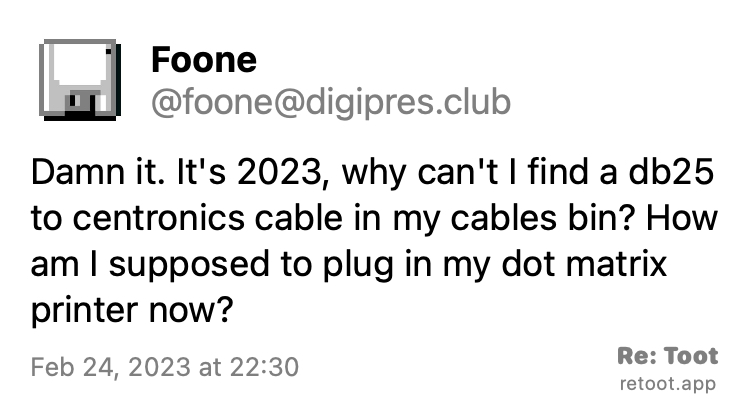
\includegraphics[keepaspectratio]{\%7B\%7Bsite.url\%7D\%7D/img/foone-dotmatrix.jpg}}
\caption{Post by Foone. ``Damn it. It's 2023, why can't I find a db25 to
centronics cable in my cables bin? How am I supposed to plug in my dot
matrix printer now?'' Posted on Feb 24, 2023 at 22:30}
\end{figure}
